\section{Implementatie Controllers}
In deze sectie overlopen we de assumpties die we hebben gemaakt over het gedrag van 
de wagen en welke bewerkingen we toegepast hebben op de invoerdata van het vage 
raamwerk. Daarna bekijken we kort de algemene lidmaatschapsfuncties, waarna we 
dieper ingaan op de specifieke implementatie van de drie verschillende 
controllers. Tenslotte kijken we naar de eventuele verschillen in de lidmaatschapsfuncties voor de individuele controllers.

\subsection{Regels}

Om de wagen doorheen de parcours te leiden hebben we enkele beschouwingen gemaakt over het gedrag van de wagen.

Ten eerste zien we dat er twee mogelijke denkwijzen zijn voor het sturen van de wagen. Ofwel laten we de wagen wegsturen van de randen van het parcours, ofwel laten we de wagen in de richting rijden naar waar deze het verste kan kijken. De eerste zal steeds een veilige route kiezen die een minimumafstand behoudt tot de grenzen van het parcours. De tweede zal echter meer sportief de binnenkant van de bocht nemen. Dit maakt de eerste manier van sturen meer geschikt voor de veilige controller terwijl de tweede voor de snelle en drift controller interessanter is.

We merken ook op dat wanneer de snelheid van de wagen omhoog gaat, de remafstand ook hoger ligt. We moeten dus ervoor zorgen dat de wagen bij hogere snelheden ook sneller zal beginnen remmen. Daarnaast kunnen bruuske bewegingen bij hoge snelheden ervoor zorgen dat de wagen begint te slippen. We zullen dus aan de hand van de sensor vooraan de wagen in combinatie met de snelheid nagaan wanneer de wagen moet beginnen remmen.

Wanneer de wagen een bocht nadert zal deze moeten vertragen. Wanneer we de 
tweede manier van sturen gebruiken, kijken we naar waar de wagen moet gaan. 
Hierbij kan een problematisch randgeval zich voordoen indien de sensoren aan 
beide zijden van de wagen ongeveer dezelfde waarden aangeven. In dit geval zullen de regels voor het sturen niet kunnen vaststellen in welke richting er gestuurd moet worden. Daarom zullen we 
de hoek van deze sensoren aanpassen indien de afstanden tot zowel de voor- als 
zij-sensoren te klein worden.

Indien de wagen begint te slippen willen we dat deze zich zal stabiliseren. We zullen in dit geval dus de versnelling van de wagen stoppen en stilaan remmen. Indien we te bruusk remmen of versnellen tijdens het remmen zullen we harder aan het slippen gaan, wat zeker niet de bedoeling is voor de veilige en snelle controllers.

Tenslotte moeten we rekening houden met de baanbreedte in combinatie met de afstanden die beide
zij-sensoren ons geven. Op het circuit van Texas zijn er bijvoorbeeld heel lange, maar ook heel
brede bochten. In Silverstone en Spa-Francorchamps is de baan daarentegen heel smal en zijn de
bochten zeer scherp. We kunnen dus niet puur afgaan op de afstanden die de
zij-sensoren aangeven om bochten op alle parcoursbreedtes te herkennen. We zullen dit moeten oplossen door deze
afstand te normaliseren. Daarom voeren we eerst een bewerking door op deze sensoren
die als resultaat een genormaliseerde waarde tussen $-1$ en $1$ oplevert, dit
resultaat noemen we \texttt{corner}. $-1$ komt overeen met een scherpe bocht
naar links, $1$ met een scherpe bocht naar rechts. Wanneer de wagen op een recht
stuk zit en dus beide zij-sensoren een gelijke waarde aangeven is het resultaat
$0$. Negatieve waarden tussen $-1$ en $0$ geven bochten naar links aan, waarbij
lagere waarden scherpere bochten zijn. Het inverse geld ook voor bochten naar
rechts. Op basis van deze \texttt{corner} waarde kunnen we dan verschillende
linguïstische termen vastleggen om scherpe, gewone en milde bochten aan te geven.

\subsection{Lidmaatschapsfuncties}

Voor de verschillende controllers gebruiken we andere lidmaatschapsfuncties. Dit 
doen we omdat bijvoorbeeld voor de veilige controller een trage snelheid lager 
zal liggen dan die in de snelle controller. Om makkelijk de vergelijking te maken hebben we de invoeren uitgezet in Figuur~\ref{fig:lidfties_in} en de uitvoeren in Figuur~\ref{fig:lidfties_out}.

\begin{figure}[h]
\centering
% KPH
  \begin{subfigure}[b]{0.32\textwidth}
    \includegraphics[width=\textwidth]{safe/carSpeedKph}
  \end{subfigure}%
  ~
  \begin{subfigure}[b]{0.32\textwidth}
    \includegraphics[width=\textwidth]{speed/carSpeedKph}
  \end{subfigure}%
   ~
  \begin{subfigure}[b]{0.32\textwidth}
    \includegraphics[width=\textwidth]{rally/carSpeedKph}
  \end{subfigure}\\
% Corner
  \begin{subfigure}[b]{0.32\textwidth}
    \includegraphics[width=\textwidth]{safe/corner}
  \end{subfigure}%
  ~
  \begin{subfigure}[b]{0.32\textwidth}
    \includegraphics[width=\textwidth]{speed/corner}
  \end{subfigure}%
   ~
  \begin{subfigure}[b]{0.32\textwidth}
    \includegraphics[width=\textwidth]{rally/corner}
  \end{subfigure}\\
% lateralVelocity
  \begin{subfigure}[b]{0.32\textwidth}
    \includegraphics[width=\textwidth]{safe/lateralVelocity}
  \end{subfigure}%
  ~
  \begin{subfigure}[b]{0.32\textwidth}
    \includegraphics[width=\textwidth]{speed/lateralVelocity}
  \end{subfigure}%
   ~
  \begin{subfigure}[b]{0.32\textwidth}
    \includegraphics[width=\textwidth]{rally/lateralVelocity}
  \end{subfigure}\\  
% frontSensor
  \begin{subfigure}[b]{0.32\textwidth}
    \includegraphics[width=\textwidth]{safe/frontSensor}
    \caption{Veilig}
    \label{fig:safe_in}
  \end{subfigure}%
  ~
  \begin{subfigure}[b]{0.32\textwidth}
    \includegraphics[width=\textwidth]{speed/frontSensor}
    \caption{Snel}
    \label{fig:speed_in}
  \end{subfigure}%
   ~
  \begin{subfigure}[b]{0.32\textwidth}
    \includegraphics[width=\textwidth]{rally/frontSensor}
    \caption{Drift}
    \label{fig:drift_in}
  \end{subfigure}\\ 
\caption{Lidmaatschapfuncties invoer}\label{fig:lidfties_in}
\end{figure}

\begin{figure}[h]
\centering
% Accel
  \begin{subfigure}[b]{0.32\textwidth}
    \includegraphics[width=\textwidth]{safe/acceleration}
  \end{subfigure}%
  ~
  \begin{subfigure}[b]{0.32\textwidth}
    \includegraphics[width=\textwidth]{speed/acceleration}
  \end{subfigure}%
   ~
  \begin{subfigure}[b]{0.32\textwidth}
    \includegraphics[width=\textwidth]{rally/acceleration}
  \end{subfigure}\\
% Brake
  \begin{subfigure}[b]{0.32\textwidth}
    \includegraphics[width=\textwidth]{safe/brake}
  \end{subfigure}%
  ~
  \begin{subfigure}[b]{0.32\textwidth}
    \includegraphics[width=\textwidth]{speed/brake}
  \end{subfigure}%
   ~
  \begin{subfigure}[b]{0.32\textwidth}
    \includegraphics[width=\textwidth]{rally/brake}
  \end{subfigure}\\
% steering
  \begin{subfigure}[b]{0.32\textwidth}
    \includegraphics[width=\textwidth]{safe/steering}
  \end{subfigure}%
  ~
  \begin{subfigure}[b]{0.32\textwidth}
    \includegraphics[width=\textwidth]{speed/steering}
  \end{subfigure}%
   ~
  \begin{subfigure}[b]{0.32\textwidth}
    \includegraphics[width=\textwidth]{rally/steering}
  \end{subfigure}\\
% scanAngle
  \begin{subfigure}[b]{0.32\textwidth}
    \includegraphics[width=\textwidth]{safe/scanAngle}
    \caption{Veilig}
    \label{fig:safe_out}
  \end{subfigure}%
  ~
  \begin{subfigure}[b]{0.32\textwidth}
    \includegraphics[width=\textwidth]{speed/scanAngle}
    \caption{Snel}
    \label{fig:speed_out}
  \end{subfigure}%
   ~
  \begin{subfigure}[b]{0.32\textwidth}
    \includegraphics[width=\textwidth]{rally/scanAngle}
    \caption{Drift}
    \label{fig:drift_out}
  \end{subfigure}\\
\caption{Lidmaatschapfuncties uitvoer}\label{fig:lidfties_out}
\end{figure}

We gebruiken de volgende invoeren:
\begin{itemize}
\item \texttt{\textbf{carSpeedKph:}} De snelheid van de wagen in km/h.
\item \texttt{\textbf{frontSensorDistance:}} De afstand van de voorkant van wagen tot de muur in meter.
\item \texttt{\textbf{corner:}} Intensiteit van de bocht, gaande van $-1$ voor een scherpe bocht naar links tot $1$ voor een scherpe bocht naar rechts. 
\item \texttt{\textbf{lateralVelocity:}} De zijwaartse snelheid van de wagen die aangeeft of de wagen al dan niet slipt.
\end{itemize}

En leggen de volgende uitvoeren vast in functie van deze invoeren:
\begin{itemize}
\item \texttt{\textbf{acceleration:}} De versnelling van de wagen van $0$ tot $1600$. Indien er geen waarde berekend wordt zal deze $0$ zijn. Deze is voor alle controllers opgedeeld in enkele termen die overeenkomen met een lage ( \texttt{slowly}), gematigde (\texttt{normal}) en snelle (\texttt{fastly}) acceleratie.
\item \texttt{\textbf{brake:}} Geeft aan hoe hard de wagen dient te remmen. Indien er geen waarde berekend wordt zal deze $0$ zijn. Deze is eveneens voor alle controllers opgedeeld in 3 termen: \texttt{slowly}, \texttt{normal} en \texttt{fastly}.
\item \texttt{\textbf{steering:}} De richting en hoe scherp er gestuurd moet worden. Deze waarde zal van $-1$ tot $1$ gaan, analoog aan de corner invoer.
\item \texttt{\textbf{scanangle:}} geeft aan wat de nieuwe hoek van de 
zijsensoren wordt. Bij de safecontroller werken we enkel met \texttt{normal} en 
\texttt{wide}, maar bij de speed- en driftcontroller breiden we deze uit met 
\texttt{narrow} en \texttt{very\_narrow} om verder vooruit te kunnen kijken.
\end{itemize}

De overige gegevens worden niet gebruikt, of worden enkel gebruikt voor de 
berekening van de inputs zoals de zij-sensoren die worden gecombineerd en 
genormaliseerd tot \texttt{corner}.

Merk op voor de uitvoer \emph{brake} dat de termen disjunct zijn in onze controllers waardoor de COG methode het gemiddelde van deze gebieden zou geven. Om ervoor te zorgen dat deze waarden toch worden opgetrokken zullen we dus in plaats van de COG formule de RM formule gebruiken in de snellere controllers. Volgens een analoge redenering hebben we geopteerd om de RM functie te gebruiken voor de acceleratie.

Alternatief hadden we deze termen discreet kunnen maken aan de hand van singletons. Hierdoor zouden we een exacte waarde kunnen opleggen aan de uitvoer. Hierdoor zou de impact van een vaag regelsysteem te gebruiken echter afgezwakt worden en zouden de controllers dus gevoeliger worden voor kleine veranderingen in de invoer.

\subsection{Veiligheid}
De veilige implementatie is een zeer eenvoudige implementatie. Om uiterst veilig
te zijn rijden we niet veel sneller dan 70 km/h, wat overeen komt met de boven grens van de term \texttt{slow} voor deze controller. Bochten nemen we afhankelijk van hun scherpte. Scherpe bochten nemen we scherp, gewone bochten nemen we
normaal en milde bochten sturen we mild in. We versnellen enkel snel wanneer de
auto traag rijdt, en remmen doen we snel wanneer een bocht binnenrijden en doen
we gestaag wanneer een bocht in de verte aankomt. Wanneer we een bocht naderen
zetten we als laatste de zij-sensoren iets wijder om een beter zicht op het soort
bocht te krijgen.

De lidmaatschapsfuncties van deze controllers is te vinden in de de linkerkolommen 
van figuren \ref{fig:lidfties_in} en \ref{fig:lidfties_out}.

Dit resulteert in de volgende regelblokken:

\begin{lstlisting}
RULEBLOCK steering
  RULE 1 : IF corner IS sharp_left_corner THEN steering IS sharp_left;
  RULE 2 : IF corner IS left_corner THEN steering IS left;
  RULE 3 : IF corner IS mild_left_corner THEN steering IS mild_left;
  RULE 4 : IF corner IS mild_right_corner THEN steering IS mild_right;
  RULE 5 : IF corner IS right_corner THEN steering IS right;
  RULE 6 : IF corner IS sharp_right_corner THEN steering IS sharp_right;
END_RULEBLOCK

RULEBLOCK speedup
  RULE 1 : IF carSpeedKph IS slow THEN acceleration IS fastly;
END_RULEBLOCK

RULEBLOCK brake
  RULE 1 : IF frontSensorDistance IS normal THEN brake IS normal;
  RULE 2 : IF frontSensorDistance IS near THEN brake IS fastly;
END_RULEBLOCK

RULEBLOCK scanangle
  RULE 1: IF frontSensorDistance is near THEN scanangle IS wide;
END_RULEBLOCK
\end{lstlisting}
\subsection{Snelheid}
We nemen voornamelijk de lidmaatschapsfuncties over van de veilige controller, maar moeten hier wel wat 
aanpassingen maken. De veilige controller versnelde nooit boven de 70 km/h. 
Daardoor moesten we geen rekening houden met hoge snelheden en dus grotere remafstanden. Met de snelle controller mikken we op hogere snelheden en zullen we dus wel moeten doen. Daarom voegen we enkele termen toe bij de 
\texttt{carSpeedKph}-invoer om op grotere snelheden te kunnen anticiperen. Deze termen zijn \texttt{very\_fast} en \texttt{hyper\_fast}. Merk hierbij op dat deze nieuwe vaagverzamelingen inclusief zijn ten opzichte van de vaagverzameling die overeen komt met de term \texttt{fast}. Dit doen we omdat we willen dat wanneer we zeer snel gaan dit nog steeds als snel beschouwd kan worden. Bovendien is de term \texttt{hyper\_fast} sterk inclusief omdat deze in de kern van de term \texttt{fast} omvat is. Voor \texttt{very\_fast} hebben we geen sterke inclusie tegenover \texttt{fast} omdat deze eerste een klein gebied buiten de kern van de laatste omvat.

Door de hogere snelheden is het belangrijk om ervoor te zorgen dat de wagen stabiel blijft. Daarom zullen we een nieuwe term toevoegen voor de \texttt{lateralVelocity}-invoer. Deze nieuwe term, \texttt{minimal}, zal aangeven dat de wagen niet alleen stabiel is maar zeer stabiel. In dit geval zal het mogelijk zijn om sterk te versnellen zonder te beginnen slippen. Daarnaast kunnen we door de verhoogde snelheid ook hogere laterale snelheden verwachten. Om deze op te vangen moeten we de lidmaatschapsfunctie van de term \texttt{drifting} uitbreiden.

Om de langere remafstanden die met deze hogere snelheden gepaard gaan moeten we vervolgens ook aanpassingen doorvoeren op de lidmaatschapsfuncties van de termen voor de \texttt{frontSensorDistance}-invoer. Hierbij zullen we geen gebruik meer maken van de term \texttt{very\_near}, waardoor we deze kunnen weglaten. Belangrijker voor deze controller is het correct inschatten van de remafstand. Derhalve breiden we de termen \texttt{far} en \texttt{very\_far} uit tot maximaal 1000 meter. Ook hier zullen we analoog aan de snelheid de term \texttt{very\_far} sterk inclusief maken ten opzichte van de term \texttt{far}.

Voor de uitvoer zullen we slechts beperkte aanpassingen moeten doen. Zo zullen we de acceleratie en het remgedrag iets scherper stellen door in plaats van de COG functie de RM functie te gebruiken. Ook verschuiven we het zwaartepunt door de grenzen tussen de termen strenger te maken.

Als laatste aanpassing aan de lidmaatschapsfuncties laten we de wagen sneller bochten ontdekken door de de \texttt{scanangle} uitvoer toe te staan te vernauwen. Dit zal gebeuren wanneer de wagen voldoen de ver kan kijken of zeer hoge snelheden haalt. Dit zal ervoor zorgen dat de wagen in mindere mate heen en weer zal schommelen bij hoge snelheden. De regels die hieruit voortvloeien staan in het \texttt{scanangle} rule-block.

De bekomen lidmaatschapsfuncties van deze controller voor de uitvoer zijn te vinden in de 
middelste kolom van Figuur~\ref{fig:lidfties_in}. De invoer is terug te vinden in dezelfde kolom van Figuur~\ref{fig:lidfties_out}.

Bij het opstellen van de regels moeten we een afweging maken tussen snelheid en 
veiligheid. We moeten snel rijden op lange stukken, maar ook rekening houden 
met de langere remweg die dit met zich meebrengt. Aan grote snelheid hebben 
kleine stuurcorrecties ook veel meer impact, dus we moeten ervoor zorgen dat we 
bij het uitvoeren van die correcties onze snelheid verlagen en niet 
versnellen tijdens deze manoeuvres om de controle over het stuur niet te 
verliezen.

Aan de regels voor de besturing van de veilige controller, in het \texttt{steering} rule-block, hebben we geen aanpassingen gedaan omdat we ervoor zorgen dat de wagen voldoende vertraagt wanneer deze een bocht nadert met de regels in het \texttt{brake} rule-block.

\begin{lstlisting}
RULEBLOCK steering
  RULE 1 : IF corner IS sharp_left_corner THEN steering IS sharp_left;
  RULE 2 : IF corner IS left_corner THEN steering IS left;
  RULE 3 : IF corner IS mild_left_corner THEN steering IS mild_left;
  RULE 4 : IF corner IS mild_right_corner THEN steering IS mild_right;
  RULE 5 : IF corner IS right_corner THEN steering IS right;
  RULE 6 : IF corner IS sharp_right_corner THEN steering IS sharp_right;
END_RULEBLOCK

RULEBLOCK speedup
  RULE 1 : IF carSpeedKph IS slow AND lateralVelocity IS stable  AND 
  frontSensorDistance IS near THEN acceleration IS slowly;
  RULE 2 : IF (carSpeedKph IS slow OR carSpeedKph IS normal) AND 
  lateralVelocity IS stable  AND 
  frontSensorDistance IS far THEN acceleration IS fastly;

  RULE 4 : IF carSpeedKph IS fast AND lateralVelocity IS minimal AND 
  frontSensorDistance IS very_far THEN acceleration IS fastly;
  RULE 5 : IF carSpeedKph IS hyper_fast AND frontSensorDistance IS NOT very_far 
  THEN acceleration IS slowly;
END_RULEBLOCK

RULEBLOCK brake
  RULE 1 : IF lateralVelocity IS drifting AND carSpeedKph IS slow THEN brake IS 
  slowly;
  RULE 2 : IF lateralVelocity IS drifting AND carSpeedKph IS NOT slow THEN 
  brake IS fastly;

  RULE 3 : IF frontSensorDistance IS near AND carSpeedKph IS normal THEN brake 
  IS normal;

  RULE 4 : IF frontSensorDistance IS NOT far AND carSpeedKph IS fast THEN brake 
  IS slowly;
  RULE 5 : IF frontSensorDistance IS NOT very_far AND carSpeedKph IS very_fast 
  THEN brake IS fastly;
  RULE 6 : IF carSpeedKph IS fast AND lateralVelocity IS NOT minimal THEN brake 
  IS normal;
  RULE 7 : IF carSpeedKph IS very_fast AND frontSensorDistance IS NOT very_far 
  THEN brake IS fastly;
END_RULEBLOCK

RULEBLOCK scanangle
  RULE 1: IF frontSensorDistance is near THEN scanangle IS wide;
  RULE 2: IF carSpeedKph IS very_fast THEN scanangle IS narrow;
  RULE 3: IF carSpeedKph IS hyper_fast THEN scanangle IS very_narrow;
END_RULEBLOCK

\end{lstlisting}
\subsection{Drift}
De driftcontroller is een meer gewaagde versie van de speedcontroller, waarbij 
er drie algemene aanpassingen zijn gebeurd. Onderstaande beschrijven we onze 
aanpassingen tegenover de hierboven besproken speedcontroller.

Ten eerste hebben we het sturen bruusker gemaakt. Hiervoor hebben we zowel de
lidmaatschapsfuncties van de termen voor \texttt{steering} iets meer richting de extremen gezet.
We hebben ook de steering regels aangepast zoals in onderstaande regelblokken te zien
zijn. In plaats van gewoon naar links te sturen in een gewone linkse bocht
oversturen we eigenlijk. Idem voor rechts. Deze toevoegingen zorgen ervoor dat
we eigenlijk té veel insturen in een bocht, waardoor de achterkant van de auto
zal uitbreken en we beginnen driften.

Dit driften moeten we natuurlijk ook tegengaan om de auto na het oversturen in
een bocht te stabiliseren. Hiervoor voegen we twee nieuwe regels toe, regel 7 en
8 in het \texttt{steering} ruleblock. Wanneer we in een bocht aan het driften
zijn zal de \texttt{corner} variabele uit deze bocht willen sturen, wat
automatisch al betekent dat de auto zal tegensturen. Dus, als we aan het driften
zijn, en de zij-sensoren zien een niet te scherpe bocht naar links/rechts dan
kunnen we concluderen dat we net hebben overstuurd in een bocht naar
rechts/links. Om dit te corrigeren sturen we in dit geval dus scherp in de bocht
die gezien wordt om het oversturen in de originele bocht tegen te gaan.

Een tweede algemene aanpassing die we hebben gemaakt is het weghalen van 
braking-rules. Om een deftige drift te kunnen uitvoeren moeten we met voldoende 
snelheid in de bocht gaan, anders breekt de achterkant van de auto niet uit. We 
willen ook niet extra gaan remmen tijdens het driften, dus ook deze regels 
halen we weg. 

Als laatste willen we uit op het eind van een drift ook extra gas geven om snel 
weg te rijden (en om wat extra rook te ontwikkelen), dus ook hiervoor is een 
extra regel toegevoegd.

De lidmaatschapsfuncties van deze controllers is te vinden in de rechterkolom 
van figuren \ref{fig:lidfties_in} en \ref{fig:lidfties_out}.

\begin{lstlisting}
RULEBLOCK steering
  RULE 1 : IF corner IS sharp_left_corner THEN steering IS sharp_left;
  RULE 2 : IF corner IS left_corner THEN steering IS sharp_left;
  RULE 3 : IF corner IS mild_left_corner THEN steering IS mild_left;
  RULE 4 : IF corner IS mild_right_corner THEN steering IS mild_right;
  RULE 5 : IF corner IS right_corner THEN steering IS sharp_right;
  RULE 6 : IF corner IS sharp_right_corner THEN steering IS sharp_right;

  RULE 7 : IF lateralVelocity IS drifting AND (corner IS mild_right_corner OR 
  corner IS right_corner) THEN steering IS sharp_right;
  RULE 8 : IF lateralVelocity IS drifting AND (corner IS mild_left_corner  OR 
  corner IS left_corner)  THEN steering IS sharp_left;
END_RULEBLOCK

RULEBLOCK speedup
  RULE 1 : IF carSpeedKph IS slow AND frontSensorDistance IS near THEN 
  acceleration IS fastly;
  RULE 2 : IF carSpeedKph IS slow AND frontSensorDistance IS far THEN 
  acceleration IS fastly;
  RULE 3 : IF carSpeedKph IS normal AND frontSensorDistance IS far THEN 
  acceleration IS fastly;

  RULE 4 : IF carSpeedKph IS fast AND lateralVelocity IS minimal AND 
  frontSensorDistance IS very_far THEN acceleration IS fastly;
  RULE 5 : IF carSpeedKph IS hyper_fast AND frontSensorDistance IS NOT very_far 
  THEN acceleration IS slowly;

  RULE 6 : IF lateralVelocity IS drifting THEN acceleration IS fastly;
END_RULEBLOCK

RULEBLOCK brake
  RULE 4 : IF frontSensorDistance IS NOT far AND carSpeedKph IS fast THEN brake 
  IS slowly;
  RULE 5 : IF frontSensorDistance IS NOT very_far AND carSpeedKph IS very_fast 
  THEN brake IS normal;
  RULE 6 : IF carSpeedKph IS fast THEN brake IS normal;
  RULE 7 : IF carSpeedKph IS very_fast AND frontSensorDistance IS NOT very_far 
  THEN brake IS fastly;
END_RULEBLOCK

RULEBLOCK scanangle
  RULE 1: IF frontSensorDistance is near THEN scanangle IS wide;
  RULE 2: IF carSpeedKph IS very_fast THEN scanangle IS narrow;
  RULE 3: IF carSpeedKph IS hyper_fast THEN scanangle IS very_narrow;
END_RULEBLOCK
\end{lstlisting}
